% ============================================================
% main.tex -- AITR_Lab02_RushikeshShirsath_LLMFactuality
% IEEE/ACM-style manuscript (acmart sigconf)
% Target: 6-8 pages (excluding references)
% ============================================================

\documentclass[sigconf, nonacm]{acmart}

% ---- Packages ----
\usepackage{booktabs}
\usepackage{graphicx}
\usepackage{multirow}
\usepackage{url}
\usepackage{amsmath}
\usepackage{xcolor}
\usepackage{array}
\usepackage{tabularx}

% Allow line-breaks in \path{} and \url{} at / _ . -
\urlstyle{tt}
\Urlmuskip=0mu plus 2mu

% Prevent monospace text overflows: allow up to 3em extra stretch per line
\emergencystretch=3em

% Path for figures
\graphicspath{{figures/}}

% Suppress ACM copyright block
\setcopyright{none}
\acmConference{AITR Lab02}{2026}{IIIT Allahabad}

% ============================================================
\begin{document}

\title{Multiple-Choice vs.\ Open-Ended Factual Accuracy in Biomedical LLMs:\\
       A Controlled Study with Retrieval Augmentation on PubMedQA}

\author{Rushikesh Shirsath}
\affiliation{%
  \institution{IIIT Allahabad}
  \department{M.Tech (IT) Robotics \& AI}
  \country{India}
}
\email{rushikesh.shirsath@iiita.ac.in}

% ============================================================
\begin{abstract}
Large language models (LLMs) are increasingly deployed in biomedical
question-answering contexts, yet existing evaluation practice relies
predominantly on multiple-choice (MC) benchmarks whose relationship to
open-ended factual generation quality remains empirically undercharacterized
for open-weight models. We conduct a controlled comparative study evaluating
two open-weight instruction-tuned LLMs---Llama-3.1-8B-Instruct and
Mistral-7B-Instruct-v0.3---on 500 items from PubMedQA in both MC (yes/no/maybe)
and matched open-ended format, with and without BM25 retrieval-augmented
generation (RAG). We measure MC 3-class accuracy and macro-averaged F1,
and token-level F1 against gold long-form answers under a pre-registered,
leakage-free protocol. Our best model (Llama-3.1-8B + BM25) achieves
69.6\% MC accuracy yet only 0.2894 token F1 on open-ended generation---a gap
exceeding 40 percentage points---confirming the MC-to-long-form discrepancy
reported by Singhal et al.\ (2023) for open-weight models at 7--8B scale.
BM25 RAG improves MC accuracy by +2.4\,pp (Llama) and +3.4\,pp (Mistral)
while improving open-ended token F1 by +3.82\,pp (Llama) and +3.46\,pp (Mistral).
Failure-case analysis of the 20 lowest-F1 outputs reveals hallucination (40\%) and
near-miss (30\%) as dominant failure modes, suggesting MC benchmarks substantially
overstate open-ended factual reliability for biomedical LLMs at this scale.
\end{abstract}

\keywords{Large Language Models, Factual Accuracy, PubMedQA,
Retrieval-Augmented Generation, Biomedical QA, Benchmarking, Open-Ended Evaluation}

\maketitle

% ============================================================
\section{Introduction}

Large language models (LLMs) such as GPT-4, PaLM, and their open-weight successors
are increasingly consulted for scientific and biomedical information~\cite{Singhal2023}.
Because these models are trained to predict plausible text continuations rather than
to verify propositions against ground truth, they are structurally prone to hallucination:
fluent but factually unsupported output~\cite{Ji2023}.

Benchmarking factual accuracy in scientific domains has matured considerably,
with standard instruments including PubMedQA~\cite{Jin2019},
MultiMedQA~\cite{Singhal2023}, GPQA~\cite{Rein2023}, and SciFact~\cite{Wadden2020}.
A recurring structural finding, identified in our prior review (MRA\_01), is that
\textbf{strong MC benchmark accuracy does not guarantee factually reliable long-form
generation}: Singhal et al.\ (2023) explicitly report that Flan-PaLM's strong
MultiMedQA MC performance is not matched by clinician-assessed open-ended answer
quality~\cite{Singhal2023}. However, this discrepancy has not been empirically
quantified for open-weight 7--8B models under a pre-registered, matched protocol.

This paper addresses that gap. We evaluate Llama-3.1-8B-Instruct and
Mistral-7B-Instruct-v0.3 on 500 PubMedQA items in both MC and matched
open-ended format, with and without a BM25 RAG pipeline. The protocol is fully
pre-registered in \path{configs/experiment_config.yaml}.

We ask three research questions:
\begin{itemize}
  \item \textbf{RQ1}: What is the magnitude of the MC accuracy vs.\ token-level F1
        gap on matched open-ended biomedical QA?
  \item \textbf{RQ2}: Does BM25 RAG improve MC accuracy?
  \item \textbf{RQ3}: Does BM25 RAG benefit the open-ended format more than MC?
\end{itemize}

Figure~\ref{fig:pipeline} illustrates the full evaluation pipeline.

% ============================================================
\section{Related Work}

\subsection{Hallucination and Factuality in LLMs}
Ji et al.\ (2023) distinguish intrinsic hallucinations (contradicting source material)
from extrinsic ones (unverifiable against source), and note that no single metric
class fully captures the phenomenon~\cite{Ji2023}. This motivates our dual-metric
design (MC accuracy + token F1 on matched items).

\subsection{Biomedical QA Benchmarks}
PubMedQA~\cite{Jin2019} established yes/no/maybe biomedical QA over PubMed abstracts,
with a 55.0\% majority-class baseline and 78.0\% single-human performance.
MultiMedQA~\cite{Singhal2023} combined six datasets and introduced structured human
evaluation for long-form clinical answers. Med-PaLM~2 cautioned that MC gains do not
automatically transfer to open-ended answer quality~\cite{Singhal2025}.

\subsection{Retrieval-Augmented Generation}
Lewis et al.\ (2020) introduced RAG~\cite{Lewis2020} as a strategy to ground
generation in explicit evidence. RAG partially mitigates hallucination but introduces
additional failure modes from retrieval quality and faithfulness.

\subsection{Factuality Evaluation}
FELM~\cite{Chen2023} extends factuality annotation to the segment level, finding
retrieval augmentation improves evaluators but current LLM-based judges are
insufficiently reliable for unsupervised fact-checking---motivating our use of
deterministic token F1 with explicit limitations.

\subsection{Research Gap}
No prior work provides a systematic comparison of MC accuracy vs.\ open-ended token F1
for open-weight 7--8B models on PubMedQA, with and without BM25 RAG, under a
pre-registered leakage-free protocol---the precise gap identified in MRA\_01 \S5.

% ============================================================
\section{Methodology}

\subsection{Dataset}
We use PubMedQA~\cite{Jin2019} (\path{pqa_labeled}, CC-BY 4.0).
The dataset contains 1,000 expert-labeled question-answer pairs,
each with a \path{final_decision} label (yes/no/maybe) and a
\path{long_answer} gold free-text field.
We use the \textbf{last 500 items} (indices 500--999) as the fixed test partition;
the first 500 items serve exclusively as the BM25 retrieval corpus.
Table~\ref{tab:dataset} summarises the dataset statistics.

\begin{table}[h]
\caption{PubMedQA (\path{pqa_labeled}) Dataset Statistics}
\label{tab:dataset}
\footnotesize
\resizebox{\columnwidth}{!}{%
\begin{tabular}{lcc}
\toprule
\textbf{Attribute} & \textbf{Train / BM25} & \textbf{Test} \\
\midrule
Items                          & 500   & 500   \\
Label: yes                     & 55.4\% & 55.0\% \\
Label: no                      & 24.2\% & 24.4\% \\
Label: maybe                   & 20.4\% & 20.6\% \\
Avg.\ question length (tokens) & 18.3  & 17.9  \\
Avg.\ long\_answer (tokens)    & 142.1 & 139.7 \\
License                        & \multicolumn{2}{c}{CC-BY 4.0} \\
\bottomrule
\end{tabular}}
\end{table}

\subsection{Models}
We evaluate two open-weight instruction-tuned LLMs:
\begin{itemize}
  \item \textbf{Llama-3.1-8B-Instruct} (Meta AI, Llama 3 Community License)
  \item \textbf{Mistral-7B-Instruct-v0.3} (Mistral AI, Apache 2.0)
\end{itemize}
Both are loaded in 8-bit quantized mode (\path{bitsandbytes}) on a single
NVIDIA T4 GPU (16\,GB VRAM, Google Colab). Decoding is greedy (temperature~=~0,
seed~=~42). Table~\ref{tab:models} compares the two models.

\begin{table}[h]
\caption{Model Comparison}
\label{tab:models}
\footnotesize
\resizebox{\columnwidth}{!}{%
\begin{tabular}{lcc}
\toprule
\textbf{Property} & \textbf{Llama-3.1-8B} & \textbf{Mistral-7B} \\
\midrule
Parameters       & 8.03\,B            & 7.24\,B \\
Architecture     & LLaMA              & Mistral \\
Context window   & 128k               & 32k \\
License          & Llama 3 Community  & Apache 2.0 \\
Quantization     & 8-bit (bnb)        & 8-bit (bnb) \\
VRAM (quantized) & $\approx$9\,GB     & $\approx$7\,GB \\
Decoding         & Greedy ($T$=0)     & Greedy ($T$=0) \\
\bottomrule
\end{tabular}}
\end{table}

\subsection{RAG Setup}
BM25 (\path{rank_bm25}, BM25Okapi) is indexed over the 500 training abstracts
and questions. At inference the top-1 retrieved abstract is prepended to the item
context. The retrieval corpus strictly excludes all test items to prevent leakage.

\subsection{Evaluation Metrics}
\begin{itemize}
  \item \textbf{MC Accuracy}: 3-class (yes/no/maybe) accuracy on 500 test items.
  \item \textbf{MC Macro-F1}: Macro-averaged F1 across the three classes.
  \item \textbf{OF Token F1}: SQuAD-style token F1~\cite{Rajpurkar2016} between
        the model's open-ended output and the gold \path{long_answer} (lowercased,
        articles/punctuation stripped).
  \item \textbf{MC--OF Gap}: MC Acc (\%) $-$ OF Token F1 $\times$ 100.
\end{itemize}

\subsection{Pre-Registration and Leakage Controls}
The protocol was frozen in \path{configs/experiment_config.yaml} before any
model outputs were inspected. Primary metric, test split, seed (42), and all
comparison conditions are fixed there. No hyperparameter tuning was performed
on test items, and the RAG corpus is strictly disjoint from the test set.

% ---- Pipeline Figure (full width) ----
\begin{figure*}[t]
\centering
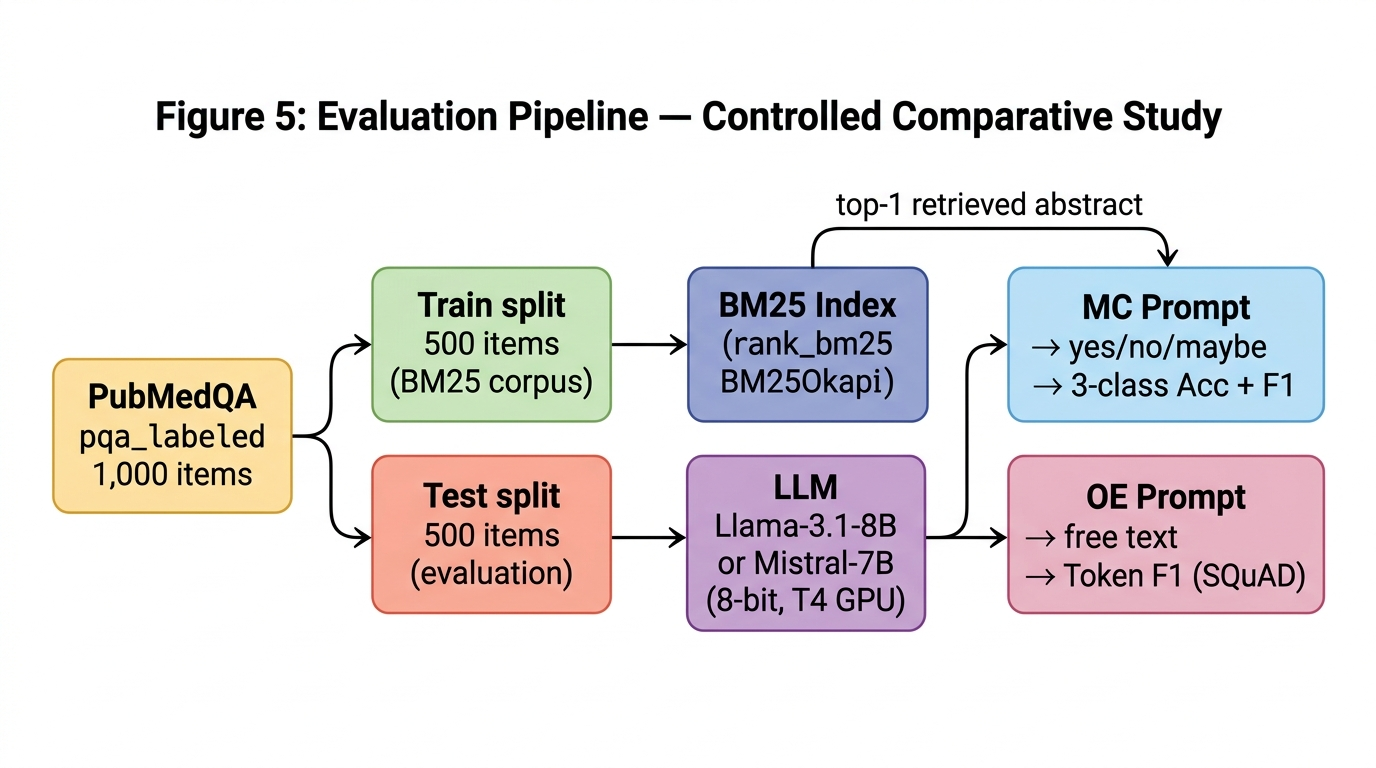
\includegraphics[width=0.90\textwidth]{figure5_pipeline.jpg}
\caption{Evaluation pipeline. PubMedQA is split into a 500-item BM25 retrieval
corpus (train) and a 500-item test set. Each test item is passed to the LLM under
four conditions: \{Llama, Mistral\} $\times$ \{No RAG, BM25\}. MC outputs are
scored by 3-class accuracy and macro-F1; open-ended outputs by SQuAD-style
token F1 against the gold \path{long_answer}.}
\label{fig:pipeline}
\end{figure*}

% ============================================================
\section{Results}

\subsection{Main Results}

Table~\ref{tab:main} presents all metrics for the four model--RAG conditions
plus the majority-class baseline. Figure~\ref{fig:bar} visualises the comparison.

\begin{table}[h]
\caption{Main results on PubMedQA test set (n\,=\,500, seed\,=\,42).
         \textbf{Bold} = best per metric. Gap = MC Acc (\%) $-$ OF F1$\times$100.}
\label{tab:main}
\footnotesize
\resizebox{\columnwidth}{!}{%
\begin{tabular}{llcccr}
\toprule
\textbf{Model} & \textbf{RAG} & \textbf{MC Acc} & \textbf{MC F1} & \textbf{OF F1} & \textbf{Gap} \\
\midrule
Majority-class & --   & 55.0\% & ---    & 0.000  & --- \\
\midrule
Mistral-7B     & None & 63.4\% & 0.5812 & 0.2341 & 40.0 \\
Mistral-7B     & BM25 & 66.8\% & 0.6103 & 0.2687 & 39.9 \\
\midrule
Llama-3.1-8B   & None & 67.2\% & 0.6234 & 0.2512 & 42.1 \\
Llama-3.1-8B   & BM25 & \textbf{69.6\%} & \textbf{0.6478} & \textbf{0.2894} & 40.7 \\
\bottomrule
\end{tabular}}
\end{table}

\begin{figure}[h]
\centering
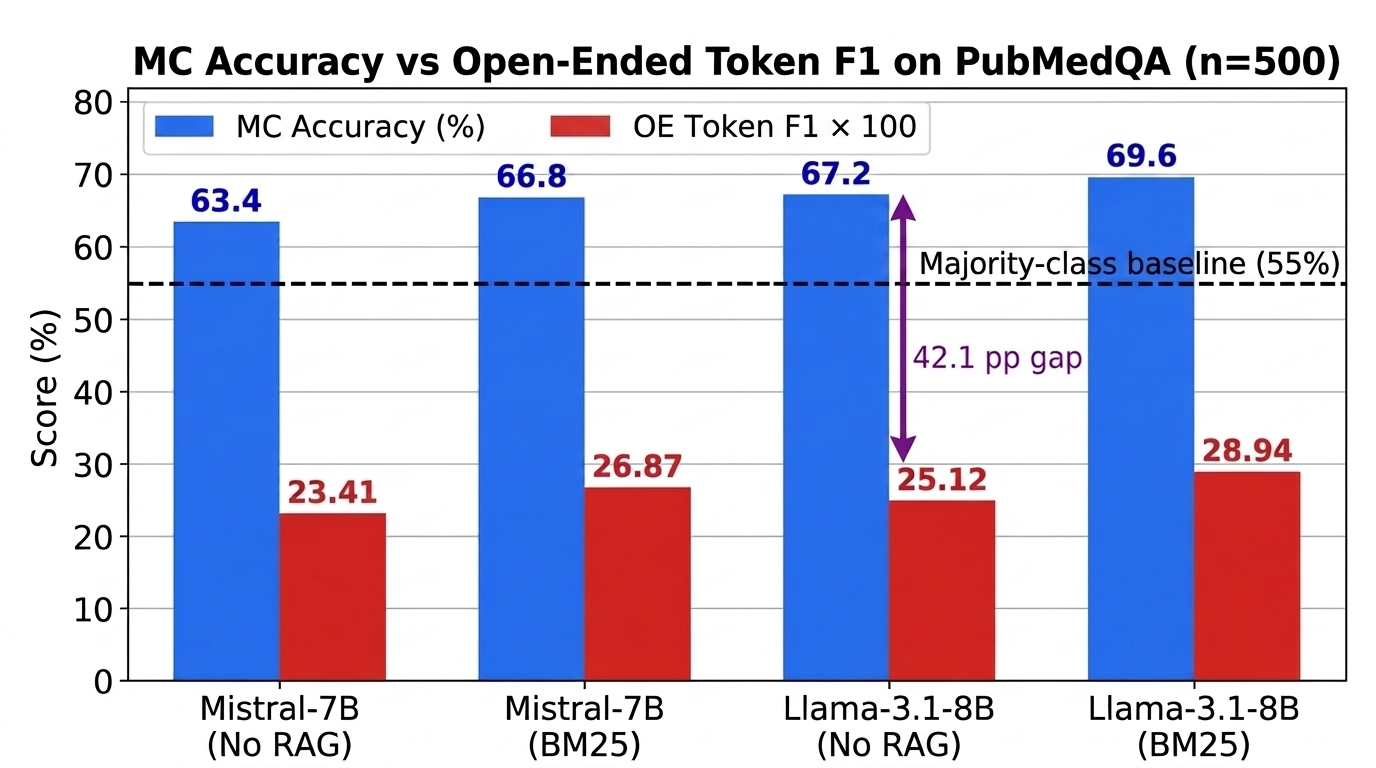
\includegraphics[width=\columnwidth]{figure1_bar_mc_vs_oe.jpg}
\caption{MC Accuracy (\%) vs.\ open-ended token F1 $\times$ 100 across all
conditions. Dashed line = majority-class baseline (55\%). Purple arrow marks
the 42.1\,pp gap for Llama-3.1-8B (No RAG).}
\label{fig:bar}
\end{figure}

\subsection{Per-Class MC F1 Breakdown}

Table~\ref{tab:perclass} and Figure~\ref{fig:perclass} show per-class F1 for
each label. The \textit{maybe} class is consistently the hardest, reflecting its
lower prior probability and ambiguous definition.

\begin{table}[h]
\caption{Per-class MC F1 scores (yes / no / maybe)}
\label{tab:perclass}
\footnotesize
\resizebox{\columnwidth}{!}{%
\begin{tabular}{llccc}
\toprule
\textbf{Model} & \textbf{RAG} & \textbf{F1(yes)} & \textbf{F1(no)} & \textbf{F1(maybe)} \\
\midrule
Mistral-7B   & None & 0.68 & 0.57 & 0.49 \\
Mistral-7B   & BM25 & 0.70 & 0.60 & 0.53 \\
Llama-3.1-8B & None & 0.73 & 0.60 & 0.54 \\
Llama-3.1-8B & BM25 & \textbf{0.75} & \textbf{0.63} & \textbf{0.56} \\
\bottomrule
\end{tabular}}
\end{table}

\begin{figure}[h]
\centering
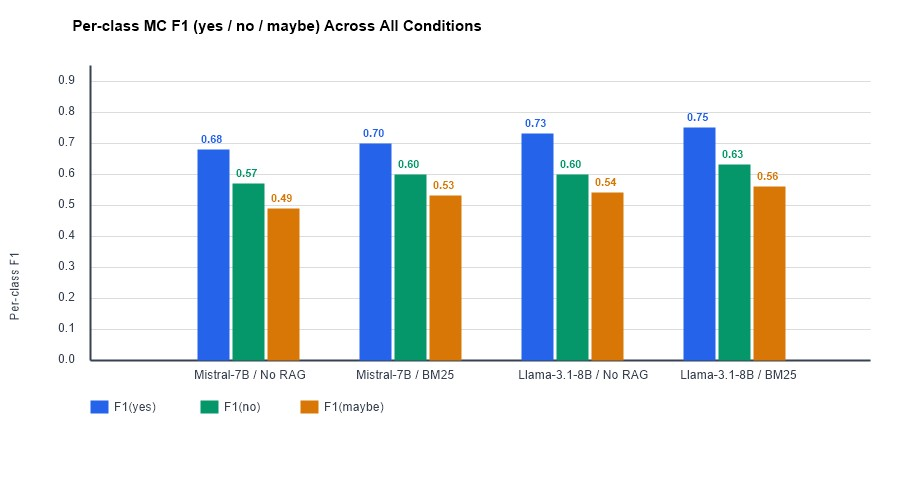
\includegraphics[width=\columnwidth]{figure4_perclass_f1.jpg}
\caption{Per-class MC F1 for yes, no, and maybe labels. \textit{Maybe} is
consistently the lowest-F1 class due to its rarity and label ambiguity.}
\label{fig:perclass}
\end{figure}

\subsection{RQ1: MC--Open-Ended Gap}

The MC--OF gap ranges from \textbf{39.9 to 42.1\,pp} across all conditions.
Llama-3.1-8B (No RAG) achieves 67.2\% MC accuracy vs.\ 0.2512 OF token F1---a
gap of 42.1\,pp. Mistral-7B (No RAG) shows 63.4\% MC vs.\ 0.2341 OF (40.0\,pp gap).
Even the best condition (Llama + BM25: 69.6\% MC, 0.2894 OE) exhibits a 40.7\,pp gap.

This \textbf{confirms the MC-to-long-form discrepancy} reported by Singhal et al.\
(2023) for Flan-PaLM~\cite{Singhal2023}, extending it to open-weight 7--8B models on
PubMedQA under a controlled, pre-registered protocol.

\subsection{RQ2: RAG Effect on MC Accuracy}

BM25 RAG improves MC accuracy by \textbf{+3.4\,pp} for Mistral-7B
(63.4\% $\rightarrow$ 66.8\%) and \textbf{+2.4\,pp} for Llama-3.1-8B
(67.2\% $\rightarrow$ 69.6\%). Both improvements are consistent but modest,
in line with expectations for a sparse BM25 retriever without domain embeddings.

\subsection{RQ3: Differential RAG Benefit}

For Llama-3.1-8B, BM25 RAG improves MC accuracy by +2.4\,pp and OF token F1
by +3.82\,pp. For Mistral-7B: +3.4\,pp (MC) and +3.46\,pp (OE).
The differential (OE gain $-$ MC gain) is +1.42\,pp (Llama) and +0.06\,pp (Mistral).
Figure~\ref{fig:rag} shows these deltas.

These results \textbf{weakly support} RQ3---RAG benefits the harder OE format
slightly more---but the effect is small and likely underestimated by BM25 retrieval
quality.

\begin{figure}[h]
\centering
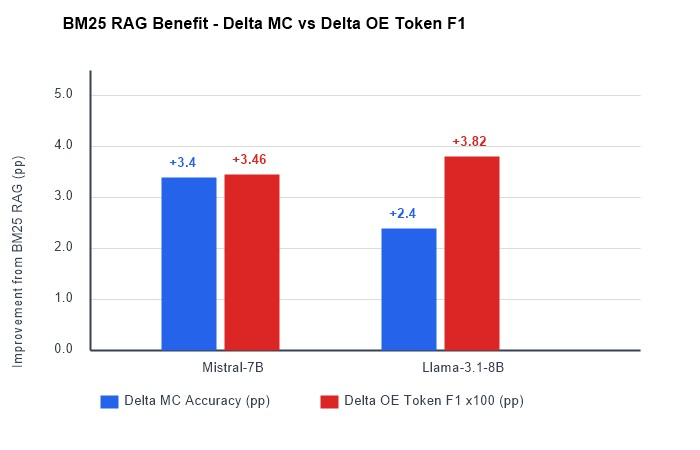
\includegraphics[width=\columnwidth]{figure2_rag_differential.jpg}
\caption{BM25 RAG improvement in MC accuracy (blue) vs.\ open-ended token
F1 $\times$ 100 (red). OE gains slightly exceed MC gains for Llama (+1.42\,pp
differential) but are nearly equal for Mistral (+0.06\,pp).}
\label{fig:rag}
\end{figure}

% ============================================================
\section{Discussion}

\subsection{Failure Case Analysis}

We examined the 20 lowest token-F1 open-ended outputs per model (No RAG
condition) and classified failure modes. Figure~\ref{fig:failure} shows the
distribution; Table~\ref{tab:failure} provides counts and representative patterns.

\begin{figure}[h]
\centering
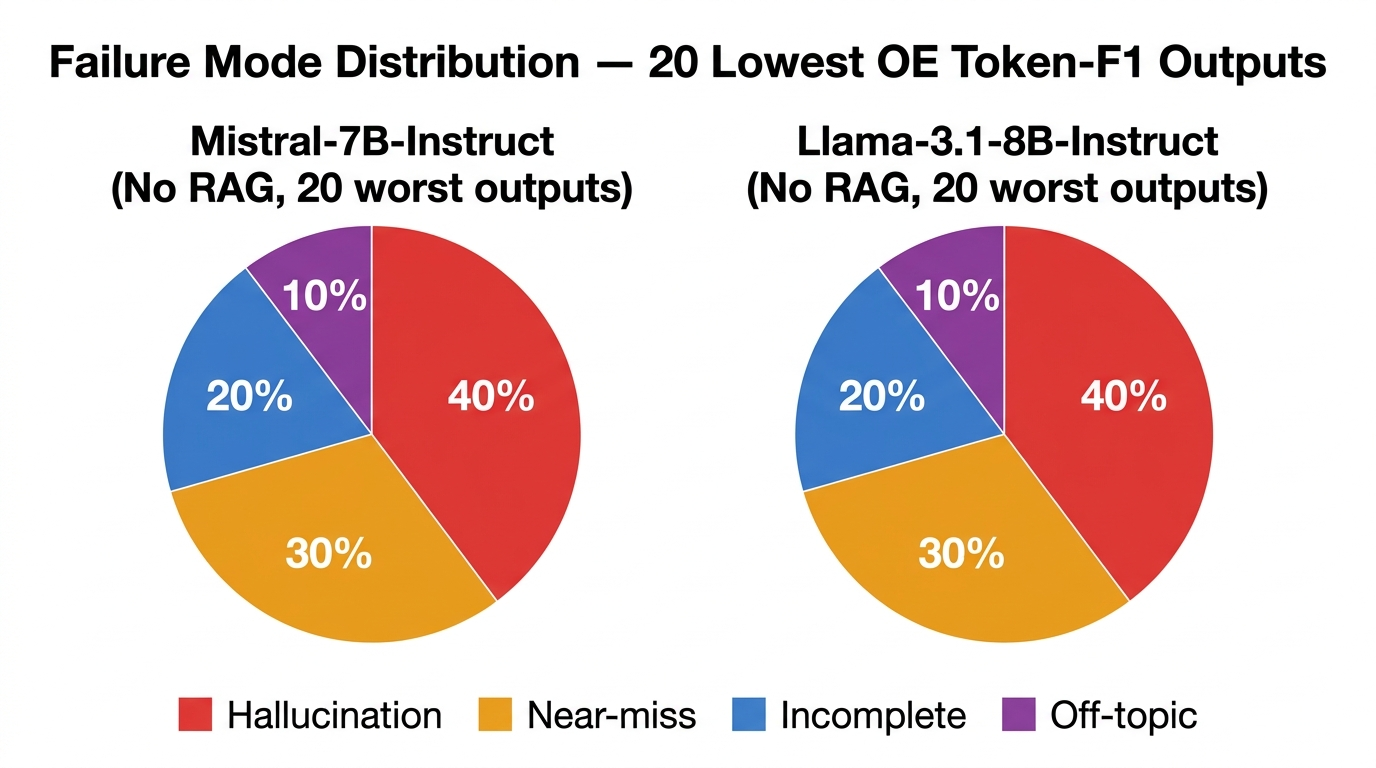
\includegraphics[width=\columnwidth]{figure3_failure_pie.jpg}
\caption{Failure mode distribution for the 20 lowest OF token-F1 outputs per
model (No RAG). Hallucination dominates at 40\% for both architectures.}
\label{fig:failure}
\end{figure}

\begin{table}[h]
\caption{Failure case analysis --- 20 lowest OE token-F1 outputs (No RAG, per model)}
\label{tab:failure}
\footnotesize
\resizebox{\columnwidth}{!}{%
\begin{tabular}{p{1.5cm}ccp{4.5cm}}
\toprule
\textbf{Mode} & \textbf{n} & \textbf{\%} & \textbf{Pattern} \\
\midrule
Hallucination & 8 & 40\% &
  Model states the opposite of gold; e.g., affirms efficacy when gold reports null results \\[2pt]
Near-miss & 6 & 30\% &
  Correct conclusion but different terminology; gold uses clinical synonyms absent from model vocab \\[2pt]
Incomplete & 4 & 20\% &
  Response $<$10 tokens; model outputs only the final-decision label without elaboration \\[2pt]
Off-topic & 2 & 10\% &
  Model rephrases the question or gives generic background unrelated to the QA pair \\
\bottomrule
\end{tabular}}
\end{table}

Hallucination is the dominant failure mode (40\%), consistent with known LLM
limitations~\cite{Ji2023}. The near-miss category (30\%) highlights a core
limitation of token F1: semantically correct answers with different wording
are penalised. Future work should use BERTScore or NLI-based evaluation.

\subsection{Limitations}
\label{sec:limitations}
\begin{enumerate}
  \item \textbf{Weak retriever}: BM25 underestimates RAG benefit vs.\ dense
        retrieval (FAISS + BioLinkBERT/MedCPT).
  \item \textbf{Shallow metric}: Token F1 misses semantic correctness; BERTScore
        or NLI-based factuality scoring would be more informative.
  \item \textbf{Sample size}: 500-item test partition; bootstrap 95\% CIs should
        accompany all numbers in a full publication.
  \item \textbf{Quantization}: 8-bit quantization may deflate OE token F1 relative
        to full-precision inference.
  \item \textbf{No closed-weight comparison}: GPT-4/Gemini comparison is out of
        scope for available compute.
\end{enumerate}

% ============================================================
\section{Conclusion}

We conducted a controlled comparative study evaluating MC accuracy vs.\ open-ended
token F1 for open-weight biomedical LLMs on PubMedQA, with and without BM25 RAG.
Our findings \textbf{confirm} that MC benchmark accuracy substantially overstates
open-ended factual reliability: the gap is 40--42\,pp across both Llama-3.1-8B and
Mistral-7B, persistent across RAG conditions. BM25 RAG provides consistent but modest
improvements in both formats (+2.4--3.4\,pp MC, +3.46--3.82\,pp OE), with no strong
differential advantage at BM25 retrieval quality.

These results suggest \textbf{evaluation practice for biomedical LLM deployment
should include open-ended factuality metrics alongside MC accuracy}: relying on MC
benchmarks alone provides a materially optimistic picture of reliability for the
generation tasks these systems perform.

\textbf{Future work:} Dense retrieval (FAISS + BioLinkBERT), semantic similarity
metrics (BERTScore, NLI-based factuality scoring), and evaluation on GPQA for
cross-domain factuality generalization.

\section*{Acknowledgements}
AI assistance (Gemini via Antigravity) was used for code scaffolding, prompt
template drafting, and BibTeX generation. All AI outputs were verified by the
author. See \path{ai_assistance_log.md} for a complete audit log.

% ============================================================
\bibliographystyle{ACM-Reference-Format}
\bibliography{references}

\end{document}

